% chap5.tex (Methodology and Result)

\chapter{Methodology and Results}

In this chapter, I have described the methodology used to forecast consumption type customer's demand. Traditionally, a single type of predictor served to predict the energy demand for all power type customers. Since each power type customers acts differently, I planned to make different forecasting mechanism for different power typed customers.

\section{The Baseline Electricity Forecasting Mechanisms}
The first baseline energy forecasting mechanism is the default prediction mechanism provided by the PowerTAC system. It exploits the fact that usage of a timeslot of a customer in a specific date is highly correlated with the day of the week and the time slot. To make a prediction it stores the average energy usage of an hour of a week. So, for each customer, it uses $24*7 = 168$ memory to remember average usages. As soon as it learns about a new usage information of an hour of a week, it updates old average using the following algorithm.


\begin{algorithm}
 
\caption{Update average usage for $customer_i$ for day d and timeslot t, $newUsage$}
\begin{algorithmic} [1]
\STATE avgUsage = get average usage of $customer_i$ at day d and time slot t
\STATE $avgUsage = 0.7 * avgUsage + 0.3 * newUsage$
\end{algorithmic}
\label{alg:updateAvgMovingAvg}
\end{algorithm}

\begin{algorithm}
\caption{forecast usage for day d and timeslot t for $customer_i$}
\begin{algorithmic} [1]
\STATE avgUsage = get average usage of $customer_i$ at day d and time slot t 
\STATE return $avgUsage$
\end{algorithmic}
 \label{alg:predictAvgMovingAvg}
\end{algorithm}

The second baseline forecasting mechanism is designed to make energy forecasts for a single customer. In general, if there are n customers in the system, we will need n energy forecasters each one trained on the data of a single customer. I went further by checking different machine learning algorithms such as M5Tree \cite{witten2005data}, Linear Regression \cite{witten2005data}, M5P rules \cite{witten2005data} and REP tree \cite{witten2005data} for each customer and picked the best performing one for each customer.

\section{Proposed Electricity Demand Forecasting Mechanism}

In this section, I will describe how I attempted to make energy demand forecaster for consumption power type customers.

\subsection{Demand Forecasting for Consumption Type Customer}
For the consumption type customers, algorithm \ref{alg:wholeAlgo} describes the proposed method of forecasting energy demand and how it was compared to the baseline methods. 


\begin{algorithm}
\caption{Make electricity demand forecasting for consumption type customer}
\begin{algorithmic}[1]
\STATE extract features for each time slot for each customer \textbf{[algorithm \ref{alg:ttxHandle}, \ref{alg:writeSlotInfo} and \ref{alg:writeWeeklyAvg} ] }

\STATE train kmeans cluster for different sizes of k \textbf{[algorithm \ref{alg:makeCluster}]} 

\STATE train linear regression classifier for each cluster and compute error \textbf{[algorithm \ref{alg:errorOfCluster}]}

\STATE pick suitable value for k by observing the errors
 
\STATE for each cluster, find the best performing predictor for that cluster \textbf{[algorithm \ref{alg:bestClassifierForCluster}]} 

\STATE train individual classifer for each customer to make the second baseline \textbf{[algorithm \ref{alg:bestClassifierIndiv}]}

\STATE evaluate performance using test data \textbf{[algorithm \ref{alg:performanceEval}]}  
\end{algorithmic}
\label{alg:wholeAlgo}
\end{algorithm}

Algorithm \ref{alg:wholeAlgo} begins with extracting information from the game log files. All the activities that occurred in a game can be found in a game log.  Activities such as buying or selling electricity occur during a time slot. At the beginning of a time slot, the system notifies the broker that a new time slot is about to begin. The system also notifies the brokers with weather forecast about the future time slots. As a time slot ends, the broker receives information about its customer's energy usage which is called tariff transaction report. Algorithm \ref{alg:ttxHandle} refers how the extraction program retrieves necessary information from tariff transaction report. As the broker gets notification of the beginning of a new time slot, the extraction program has all the information related to energy usage and weather data of the previous time slot available by this time. The extractor program extracts the following features for each time slot -
 
\begin{itemize}
  \item Temperature
  \item Cloud Cover
  \item Wind Speed
  \item Average of the Slot
  \item Standard Deviation of the Slot
\end{itemize}

Algorithm \ref{alg:writeSlotInfo} shows the procedure of writing the information of the known time slot's information in training instance file. Once the simulation ends, the extraction program knows the average energy usage of all the customers during a week. The extraction program writes all the 168 hourly averages of a week to a file. This is explained in algorithm \ref{alg:writeWeeklyAvg}. 

%feature extraction
\begin{algorithm}[!h]
\caption{extract information from transactionReport sent to broker after each time slot through TariffTransactionHandler call back method}
\begin{algorithmic} [1]
\STATE timeSlot = get time slot from transactionReport
\STATE customerName = get customer name from transactionReport
\STATE energyUsed = get energy used from trom transactionReport
\STATE addUsage(customerName, timeSlot, energyUsed)
\end{algorithmic}
 \label{alg:ttxHandle}
\end{algorithm}

%write extracted features
\begin{algorithm} [!h]
\caption{write extracted data after timeSlot update message received from TimeSlotUpdateHandler call back method}
\begin{algorithmic} [1]
\STATE knownTimeSlot = timeSlot - 1
\FOR{each customer}
\STATE day = get day of knownTimeSlot
\STATE hour = get hour of knownTimeSlot
\STATE statisticalData = get statistics of the customer of day and hour
\STATE weatherData = get weather data of knownTimeSlot
\STATE trueUsage = get true usage of customer in knownTimeSlot
\STATE trainingInstance = create training instance by combining statistical data, weather data and true usage 
\STATE writeToFile(trainingInstance)
\ENDFOR
\end{algorithmic}
\label{alg:writeSlotInfo}
\end{algorithm}

%write weekly avg of each customer
\begin{algorithm} [!h]
\caption{write average electricity usage of the customers of each hour of the week}
\begin{algorithmic} [1]
\REQUIRE information of all timeslots has been received
\FOR{each customer}
    \STATE trainingInstance = create empty training instance
    \FOR{each day of week}
        \FOR{each hour of day}
            \STATE averageUsage = get average usage of day and hour of customer
            \STATE append averageUsage to the trainingInstance
        \ENDFOR
    \ENDFOR
    \STATE writeToAvgUsageFile(trainingInstance)
\ENDFOR
\end{algorithmic}
\label{alg:writeWeeklyAvg}
\end{algorithm}


Next, all the average weekly usages are combined together to make training set for the clustering algorithm. I have used k-means \cite{witten2005data} clustering algorithm to cluster the  training set. I have trained clusters of sizes 4, 5, 6, 7, 8, 9, 10 and 11. Algorithm \ref{alg:makeCluster} describes the procedure of making clusters from the training instances. Once a k-means of cluster size k is made, a program groups the hourly usages of the customers in the same cluster and combines them to make training set for  machine learning classifier. This training set is used to train linear regression classifier. To test the performance of the classifiers, I have separated five game logs and they were not used for training purposes. Algorithm \ref{alg:errorOfCluster} describes how the cluster based predictor's performance was evaluated. 

%make cluster

\begin{algorithm}
\caption{create kmeans cluster of size k from weekly usage training instance file}
\begin{algorithmic} [1]
\STATE data = load weekly average usage file
\STATE kmeansCluster = build kmeans cluster of size k based on data
\STATE save kmeansCluster
\end{algorithmic}
\label{alg:makeCluster}
\end{algorithm}


%observe error of each cluster
Based on the errors observed from different k-means cluster based forecasting mechanisms, I fixed the number of clusters. Once the number of the clusters was fixed, a program creates several machine learning predictors to see which one performs best for a given cluster. The machine learning classifiers that were tried out are linear regression \cite{witten2005data}, M5P rules \cite{witten2005data}, M5 Tree\cite{witten2005data}, REP tree\cite{witten2005data}. In the runtime, a customer will be grouped in a cluster based on its weekly usage. Once the program knows the cluster assigned to a customer, the program will load the corresponding demand forecaster to make electricity demand forecast about the customers.

%find size of k
\begin{algorithm}[!h]
\caption{find error of kmeans clusters of different size}
\begin{algorithmic} [1]

\FOR{each cluster size k}
    \STATE get the kMeansCluster of size k
    \FOR{cluster in KMeansCluster}
        \STATE combine slot based training instances of that cluster
        \STATE train linear regression classifier based on the combined data
        \STATE save the classifier for cluster
    \ENDFOR
\ENDFOR

\FOR{each training instance}
    \STATE compute error of the instance using each kMeansCluster
\ENDFOR
\end{algorithmic}
\label{alg:errorOfCluster}
\end{algorithm}

%find best classifier for cluster of size k
\begin{algorithm} [!h]
\caption{find best classifiers of each cluster of kmeans cluster of size k}
\begin{algorithmic} [1]
\FOR{each cluster in kMeansCluster}
    \STATE combine slot based data of the all the customers in cluster
    \STATE train available classifiers on the combined data using 10 fold cross validation
    \STATE choose the classifier with minimum error
    \STATE save the classifier for making demand forecasting for cluster
\ENDFOR 
\end{algorithmic}
\label{alg:bestClassifierForCluster}
\end{algorithm}


%%% begin from here
At this phase, I have the proposed cluster-based customer's demand forecaster. Next, the baseline predictor that needs a machine learning classifier for each customer is built. At first, the training instances are combined based on the name of the customer. This means for n customers n training set is constructed, each of the training set has only the information of a single customer. A training set related to a customer is used to create machine learning classifiers for that customer. Several classifiers had been tried out to figure out which classifier performs the best for a customer. The best performing classifier was chosen to predict about a customer. Algorithm \ref{alg:bestClassifierIndiv} explains the procedure of getting the best classifier.

%find best classifier for individual customers
\begin{algorithm}[!h]
\caption{find best classifiers created for each individual customer}
\begin{algorithmic} [1]
\FOR{each customer}
    \STATE combine all slot based training instance of the customer
    \STATE train available classifiers on the combined data using 10 fold cross validation
    \STATE choose the classifier with minimum error
    \STATE save the classifier for making prediction about the customer
\ENDFOR 
\end{algorithmic}
\label{alg:bestClassifierIndiv}
\end{algorithm}

The next phase is to test the performance of the proposed and baseline methods. For testing, I had used five game logs that were not used for training purposes. For each test instance, all three methods output was observed to figure out the performance. Algorithm \ref{alg:performanceEval} shows the mechanism of testing.

%Testing
%Testing
\begin{algorithm}
\caption{performance evalulation of each method}
\begin{algorithmic} [1]
\FOR{each test instance}
    \STATE classify the test instance using moving average usage \textbf{[algorithm \ref{alg:predictAvgMovingAvg}]}
    \STATE classify the test instance using individual prediction mechanism
    \STATE classify the test instance using cluster based predictor
    \STATE calculate and accumulate errors of each mechanism \textbf{[algorithm\ref{alg:errorCalculation}]}
    \STATE update moving average baseline predictor based on the information from the test instance \textbf{[algorithm \ref{alg:updateAvgMovingAvg}]}
\ENDFOR 
\STATE find average error from the accumulated errors for each forecasting mechanism
\end{algorithmic}
\label{alg:performanceEval}
\end{algorithm}
%calculate error
\begin{algorithm} [!h]
\caption{calculate error from the predicted value and the true value}
\begin{algorithmic} [1]
\STATE absoluteError = abs(predictedValue - trueValue)
\STATE relativeAbsoluteError = (absoluteError / trueValue ) * 100 \%
\end{algorithmic}
\label{alg:errorCalculation}
\end{algorithm}

\section{Result}
The following subsections describe the results at each stage of experiments. The stages are finding optimal number of clusters. Once the number of clusters has been fixed, different classifier needs to be made for each cluster to see which one makes the best forecast for a particular cluster. After that, the baseline predictor that needs a classifier for each customer needs to be built. At this point, for each customer several classifier has been tried out to see which classifier makes best demand forecast about that customer. After that, the proposed mechanism has been tested against the two baseline demand forecasting methods.

\subsection{Finding number of clusters}

At first, I have segmented the customer using KMeans clustering algorithm with cluster sizes = 4, 5, 6, 7, 8, 9, 10 and 11. For KMeans with size k, we will have k clusters. For each of the k clusters, I had a linear regression predictor. I observed the relative percentage error and absolute average the above cluster sizes. It turned out that the size of the cluster does not have a big impact on the prediction performance. To keep things simple, I have decided to choose Kmeans cluster of size 4. When k = 4 was chosen, table \ref{table:clusterAss} shows the cluster assignment for each customer. It can be seen that, cluster-0 held most of the offices, cluster 2 held most of the village types, cluster 3 held the medical center, cluster 1 held large housing such as brooksidehomes, centerville homes and large offices such as downtown offices and centerville offices.


\begin{table}[h!]
\centering
\caption{Assigned cluster for each customer}
\begin{tabular}{|c| c|} 
 \hline
 Customer Name & Assigned Cluster Number \\ [0.5ex] 
 \hline
BrooksideHomes &	0 \\
CentervilleHomes & 0 \\
DowntownOffices & 1	\\
EastsideOffices &	1 \\
OfficeComplex 1 NS Base &	0 \\
OfficeComplex 1 SS Base &	0 \\
OfficeComplex 2 NS Base &	0 \\
OfficeComplex 2 SS Base &	0 \\
Village 1 NS Base &	2 \\
Village 1 RaS Base &	2 \\
Village 1 ReS Base &	2 \\
Village 1 SS Base &	2 \\
Village 2 NS Base &	2 \\
Village 2 RaS Base &	2 \\
Village 2 ReS Base &	2 \\
Village 2 SS Base &	2 \\
MedicalCenter@1	& 3 \\ [1ex] 
 \hline
\end{tabular}
\label{table:clusterAss}
\end{table}

\subsection {Finding best predictor for each cluster}
Once the features are extracted, I have tried out  M5Tree, Linear Regression, M5P rules and REP tree machine learning classifiers to see which one performs the best for each of the 4 clusters. Figure \ref{fig:cluster-0-predictors}, \ref{fig:cluster-1-predictors}, \ref{fig:cluster-2-predictors}, \ref{fig:cluster-3-predictors} show that M5P, M5P, REPTree and M5RULES are the best predictors for cluster 0, 1, 2 and 3 respectively.

%%trial 1
\begin{figure}
\centering
\begin{minipage}{.5\textwidth}
  \centering
  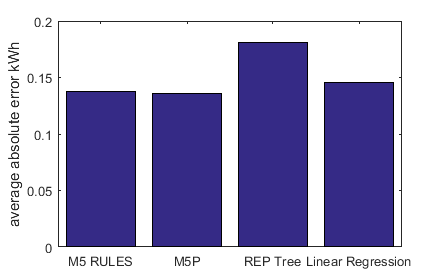
\includegraphics[width=\linewidth]{cluster-0-diff-classifier-avg-abs.png}
  \caption{cluster 0 avg absolute error of 4 classifiers}
  \label{fig:cluster-0-predictors}
\end{minipage}%
\begin{minipage}{.5\textwidth}
  \centering
  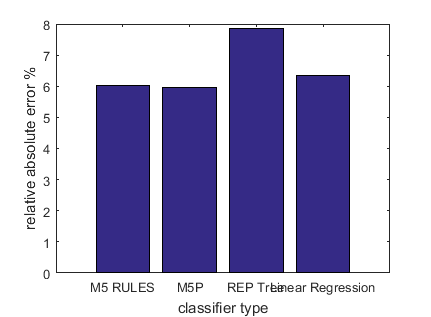
\includegraphics[width=\linewidth]{cluster-0-diff-classifier-relative-abs.png}
  \caption{cluster 0 avg relative absolute error of 4 classifiers}
\end{minipage}

\centering
\begin{minipage}{.5\textwidth}
  \centering
  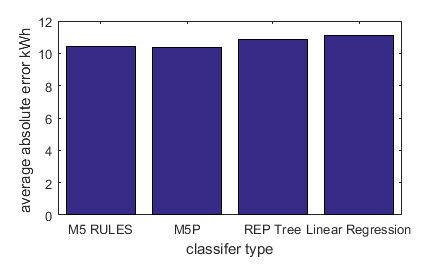
\includegraphics[width=\linewidth]{cluster-1-diff-classifier-avg-abs.png}
  \caption{cluster 1 avg absolute error of 4 classifiers}
  \label{fig:cluster-1-predictors}
\end{minipage}%
\begin{minipage}{.5\textwidth}
  \centering
  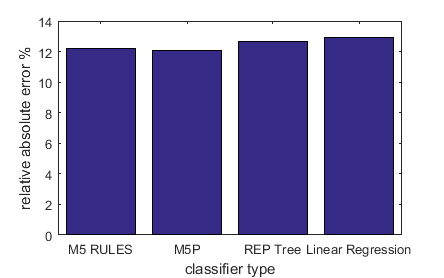
\includegraphics[width=\linewidth]{cluster-1-diff-classifier-relative-abs.png}
  \caption{cluster 1 avg relative absolute error of 4 classifiers}
\end{minipage}

\end{figure}
%% trial 1 end

%% trial 2
\begin{figure}

\centering
\begin{minipage}{.5\textwidth}
  \centering
  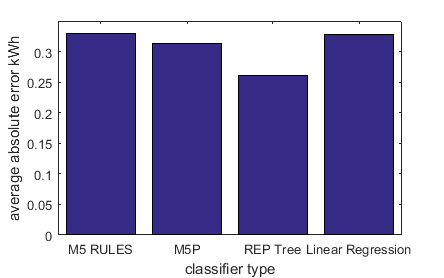
\includegraphics[width=\linewidth]{cluster-2-diff-classifier-avg-abs.png}
  \caption{cluster 2 avg absolute error of 4 classifiers}
  \label{fig:cluster-2-predictors}
\end{minipage}%
\begin{minipage}{.5\textwidth}
  \centering
  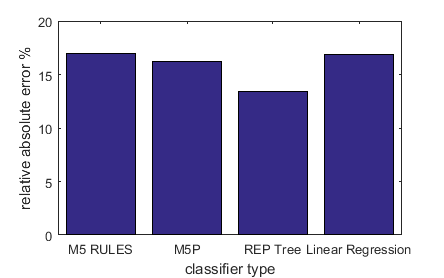
\includegraphics[width=\linewidth]{cluster-2-diff-classifier-relative-abs.png}
  \caption{cluster 2 avg relative absolute error of 4 classifiers}
\end{minipage}

\centering
\begin{minipage}{.5\textwidth}
  \centering
  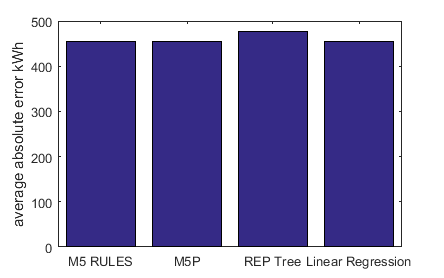
\includegraphics[width=\linewidth]{cluster-3-diff-classifier-avg-abs.png}
  \caption{cluster 3 avg absolute error of 4 classifiers}
  \label{fig:cluster-3-predictors}
\end{minipage}%
\begin{minipage}{.5\textwidth}
  \centering
  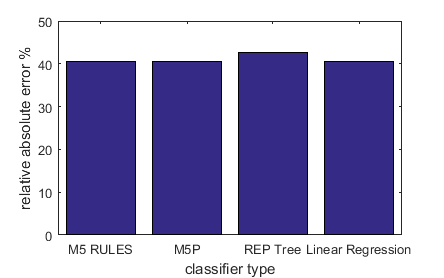
\includegraphics[width=\linewidth]{cluster-3-diff-classifier-relative-abs.png}
  \caption{cluster 3 avg relative absolute error of 4 classifiers}
\end{minipage}

\end{figure}
%% trial 2 end

The next step is to find the best classifiers for each of the customers. Based on the data from each of the customers, the four types of classifiers described in previously were tried out. For each customer, the following classifiers performed the best. 

\begin{table}[h!]
\centering
\caption{Best individual predictor for each customer}
\begin{tabular}{|c| c|} 
 \hline
 Customer Name & Best Predictor Type \\ [0.5ex] 
 \hline
BrooksideHomes &	M5P \\
CentervilleHomes &	M5P \\
DowntownOffices &	M5P \\
EastsideOffices &	M5P \\
OfficeComplex 1 NS Base &	LinearRegression \\
OfficeComplex 1 SS Base &	LinearRegression \\
OfficeComplex 2 NS Base &	LinearRegression \\
OfficeComplex 2 SS Base &	LinearRegression \\
Village 1 NS Base &	M5P \\
Village 1 RaS Base &	LinearRegression \\
Village 1 ReS Base &	M5P \\
Village 1 SS Base &	M5P \\
Village 2 NS Base &	LinearRegression \\
Village 2 RaS Base &	M5P \\
Village 2 ReS Base &	M5P \\
Village 2 SS Base &	M5P \\
MedicalCenter@1	& M5P \\ [1ex] 
 \hline
\end{tabular}
\label{table:1}
\end{table}

The figure \ref{fig:indiv-cutomer-best-predictor-error} shows error percentage of each of the predictors type for each of the customer types.

\begin{figure}[h!]
  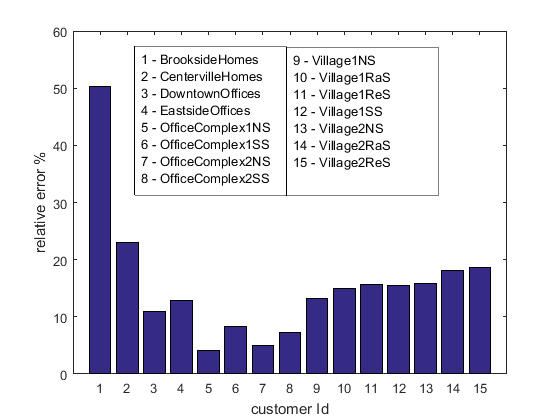
\includegraphics{relativeErrorIndivPredictor.png}
  \caption{Performance of the best classifier for each customer type. Customer Medical center was excluded as it was showing huge error. }
  \label{fig:indiv-cutomer-best-predictor-error}
\end{figure}

Finally, the cluster based forecasting and the two baselines were tested with data extracted from 5 test files that were not used for training. From Figure \ref{fig:prediction-scheme-vs-error}, we can see that cluster based prediction mechanism performed almost as good as the mechanism where n predictors are needed for n customers. And it did well than the default moving average prediction scheme.



\begin{figure}[h!]
\centering
\begin{minipage}{.5\textwidth}
  \centering
  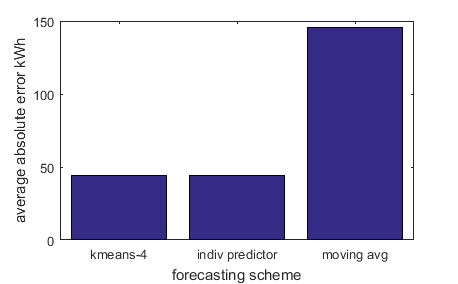
\includegraphics[width=\linewidth]{final-avg-abs-error.png}
  \caption{average absolute error}
  \label{fig:prediction-scheme-vs-error}
\end{minipage}%
\begin{minipage}{.5\textwidth}
  \centering
  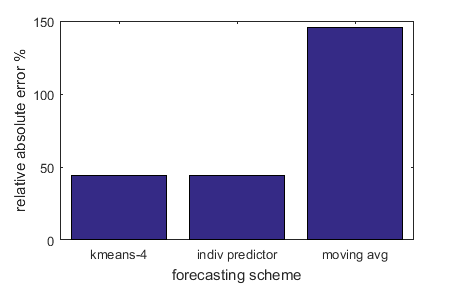
\includegraphics[width=\linewidth]{final-relative-abs-error.png}
  \caption{average percent relative absolute error}
\end{minipage}

  
\end{figure}